\subsection{Dictionary Based Algorithms}
\label{SubsectionDictionary}
As previously discussed, shapelet algorithms are very good at identifying unique subseries which can be related to class labels either by their presence or absence.
This technique although very helpful for some problems, but it can deceived if the class labels are defined by the relative frequency of some patterns and not just the a single match \cite{large2018bop,bagnall2017great}.
Dictionary based algorithms is a family of algorithms that uses the frequency of words as the foundation of finding discriminatory features of classes \cite{middlehurst2019scalable}.
They can address this type of problems by tracking the frequency counts of repeating patterns, which makes them resilient to noisy data \cite{shifaz2020ts}.
To achieve this, dictionary based algorithms transform time series data into words; to reduce their dimensionality and approximate their values.
Then based on the distribution of the words they measure similarity between instances \cite{lin2012rotation,schafer2015boss}.

In general, the process of dictionary based classifiers involves using a sliding window, of some length $w$, over the data.
Then for each window, an approximation process is carried out to reduce its length to from $w$ to a shorter length $l$ \cite{bagnall2020tale}.
A quantization process then follows; to discretize the real values into words by assigning letters to each value.
When all the windows are finished, the number of occurences of words is calcualted and each time series is represented by a histogram \cite{shifaz2020ts}.
In the end, similarity between instances is calculated based on similarity between histograms.

Differrent dictionary based algorithms apply different approximation and discretization techniques.
For example two of the older algorithms; Bag of Patterns (BoP) \cite{lin2012rotation} and Symbolic Aggregate Approximation-Vector Space Model (SAX-VSM) \cite{senin2013sax}
use an approximation method called Symbolic Aggregate Approximation (SAX) \cite{lin2007experiencing}.
SAX extends Piecewise Aggregate Approximation (PAA), a method that divides a time series into equal consecutive segments and concatenates their means \cite{shifaz2020ts}.
Then to transform the series into words, it creates break points using quantiles from the normal distribution.
In addition to using SAX, SAX-VSM merges it with the vector space model from the Information Retrieval domain.
The major difference between BOP and SAX-VSM, is that SAX-VSM calcualtes its frequencies on the class level rather than on the series level.
Then applies weighting using inverse document frequency \cite{bagnall2017great}.

On the other hand, the newer algorithms; BOSS \cite{schafer2015boss}, BOSS-VS \cite{schafer2016scalable} and WEASEL \cite{schafer2017fast}
use another method which is called Symbolic Fourier Approximation (SFA) which approximates data using coefficients of Discrete Fourier Transformation (DFT).
Then apply an adaptive technique called Multiple Coefficient Binning (MCB) to quantize the data.
These two techniques; SFA and MCB, will be discussed in more details in the next parts.

\subsubsection{BOSS}
\label{SubsubsectionBOSS}
Bag of SFA Symbols (BOSS) is a dictionary based algorithm that was introduced by \cite{schafer2015boss} in 2015.
Like the previous dictionary based classifiers, BOP and SAX-VSM,
BOSS also used a windowing technique to extract patterns from the data and transform them into words, but it had other significant differences to them \cite{bagnall2017great}.
BOSS was concerned with the issue of dealing with noisy data which, at that time, received little attention; due to the common practice of
either using raw data directly or handling noise in a preprocessing stage. The goal was to introduce an algorithm faster than its rivals of the same group,
robust for existence of noise in the data and competitive with existing TSCA.

% General description of BOSS Model
The BOSS model is divided into several steps, figure \ref{Img:BossFlow} shows these steps.
In the beginning, it passes a window of size w over the time series to extract substructures.
Each of the extracted windows is then normalized; to obtain amplitude invariance.
While obtaining offset invariance by subtracting the mean value for each window is data set specific and can be decided upon based on a parameter.
Then the substructures are quantized using SFA transformations; which transforms the data into unordered words.
This helps further reduce the noise in the data by making it phase shift invariant and makes it possible to apply string matching algorithms on the data.
Since some data sets might happen to have long constant signals, this will lead to SFA transformations of their windows to produce the same words multiple times
and cause higher weights to be assigned for them. BOSS applies a numerosity reduction technique adopted from \cite{lin2007experiencing,lin2012rotation}
that ignores multiple sequential occurences of the same word.
Finally, time series instances can be compared for differences using the noise reduced substructures by applying a customized distance measure inspired by Euclidean distance.
We will, briefly, discuss the main components that are used for each of the previously mentioned steps.

\begin{figure}[!htbp]
    \captionsetup{justification=raggedright}
    \centering
    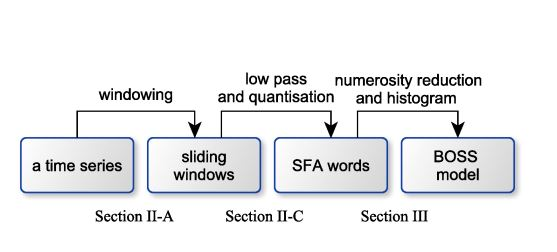
\includegraphics[scale = 0.5]{BossFlow.JPG}
    \centering
    \caption{The BOSS workflow \cite{schafer2015boss}}
    \label{Img:BossFlow}
\end{figure}

% Windowing
To extract the substructures from a given time series instance $T = [t_{1},t_{2},...t_{n}$],
a windowing function is used to split it into fixed sized windows $S_{i;w} = (t_{i},,...t_{i+w-1}$), each of them is of a size $w$.
The total number of windows that can be created for a time series of length n is $n-w+1$, and each consecutive windows overlap on $w-1$ points.
In order to achieve offset and amplitude invariance, each window is z-normalized by subtracting the mean from its original values and then dividing the difference
by the standard deviation.
\begin{equation}
    windows(T,w) = \{ S_{1;w}, S_{2;w}, ...,  S_{n-w+1;w} \}
\end{equation}

%SFA
After running the windowing function, the real values of the time points inside the windows are transformed into words using SFA \cite{schafer2012sfa}.
SFA is an alternative way of representing time series data, that instead of using real values, uses a sequence of symbols which are referred to as SFA words based on a predefined alphabet of specific length.
SFA accomplishes two things; low pass filtering through removal of noisy components from the data and string representation which allows for the use of string matching algorithms.

%   SFA Step 1
For SFA to achieve its goals, two main operations have to be carried out; approximation and quantization.
Approximation is the process of representing a specific signal of length n using another signal of lower length l.
This is achieved using Discrete Fourier Transformation (DFT); a transformation technique which is applied to a singal represented by a sequence of equally spaced values
into a sequence of coefficients of complex sinusoid waves ordered by their frequencies \cite{liao2017separable}. The higher coefficients in a DFT refer to data with
with rapid changes, which can be considered as noise in the signal and thus ignored. So considering only the first l $\ll$ n coefficients acts as a low pass filter for noise
producing a smoother signal.

%   SFA Step2
Quantization also helps reduce noise by splitting the frequency domain into equi-depth bins, then maps each of the Fourier real and imaginary coefficients into a bin.
BOSS utilizes Multiple Coefficient Binning (MCB), an adaptive technique that minimizes the loss of information which is a side effect of quantization.
After the approximation step, a matrix is built from the Fourier transformations of the training data set using only the first $\frac{l}{2}$ coefficients,
including both the real and imaginary values for each coefficient. Then using an alphabet $\Sigma$ of size c, MCB creates for each columm of the matrix c+1 break points
using equi-depth binning. During classification, to acquire the SFA word for a Fourier transformed time series, a lookup is done on the precomputed MCB bins and
a word is assigned if the value falls within it bin's boundaries. Figure \ref{Img:BOSS_SFA} demonstrates the approximation and quantization processes in BOSS.

% BOSS distance
After the transformation of instances to SFA words, BOSS uses a customized distnace measure referred to as BOSS distance; to measure the similarity between the transformed instances.
BOSS distance is a variation of Euclidean distance, which compares instances based on the histograms formed from their transformed forms. The appearence of the same SFA words in both
instances, is considered to be a notion of similarity. While the absence of SFA words might be caused by one of two reasons; the absence of some substructures from either instances,
or due to the presence of noise which disfigures the time series. Instances under BOSS distance are compared based on shared SFA words only, thus excluding words of frequencies equal to 0.
BOSS distance as noted by \cite{schafer2015boss} is:

Given two time series instances $T_{1}$ and $T_{2}$ and their corresponding
BOSS histograms $B_{1}$ : $\Sigma\textsuperscript{l}$ $\to$ $\mathbb{N}$
and $B_{2}$ : $\Sigma\textsuperscript{l}$ $\to$ $\mathbb{N}$, where l is the word length and $\Sigma$ is an alphabet of size c. Their BOSS distance is:
\begin{equation}
        D(T_{1},T_{2}) = dist(B_{1},B_{2})
\end{equation}
where
\begin{equation}
    dist(B_{1},B_{2}) = \sum_{a \epsilon B_{1};B_{1}(a)>0}^{} [B_{1}(a) - B_{2}(a)]\textsuperscript{2}
\end{equation}

\begin{figure}[!htbp]
    \captionsetup{justification=raggedright}
    \centering
    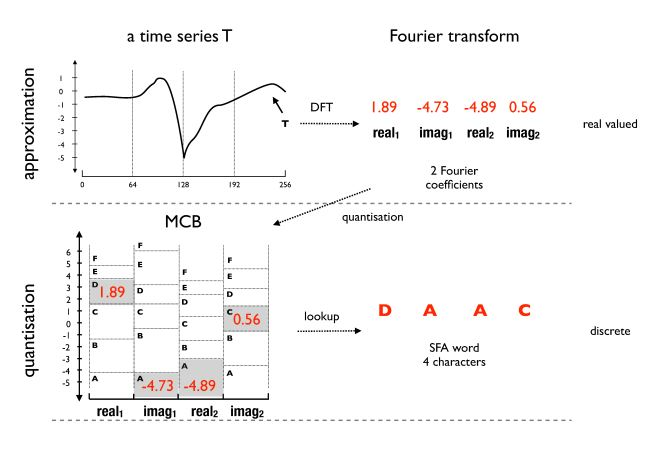
\includegraphics[scale = 0.5]{BOSS_SFA.JPG}
    \centering
    \caption{A time series is (a) approximated (low pass filtered) using DFT and (b) quantised using MCB resulting in the SFA word DAAC \cite{schafer2015boss}}
    \label{Img:BOSS_SFA}
\end{figure}

% Classifying with BOSS
Each single BOSS classifier utilizes 1-NN approach along with its BOSS model. The reason behind using 1-NN is that it is a simple technique 
that doesn't add to the parameters of the model, but rather proved to be a robust one. When classifying a query instance, BOSS searches
for the nearest neighbor in a sample of candidates by chossing the closest instance based on the BOSS distance.

Finally, BOSS Ensemble is introduced as an ensemble of multiple BOSS classifiers. While a fixed window length is used over time series instances for BOSS classifier,
BOSS Ensemble considers representing each time series instance by ensembling multiple BOSS classifiers, each of a different window length.
When the training data is fitted, BOSS Ensemble acquires a group of scores for each of the different window lengths.
To classify a query instance, BOSS Ensemble acquires the best accuracy score from the score sets returned during training.
Then considers all window lengths that obtained accuracies within a factor of the best accuracy score.
Each of the considered windows predicts a class label for the query instance using 1-NN. Majority voting is applied and the most dominant
class label is assigned.

In \cite{middlehurst2019scalable}, some enhancements were introduced to BOSS.
These included randomising the parameter settings, subsampling training data for each classifier,
adding a voting scheme to assign weights to classifiers based on the probability distribution from cross validation on training dataset,
fixing the number of classifiers and adding a time contract.

The new enhanced version of BOSS is named the Contractable BOSS or CBoss.
In the contractable BOSS, the ensemble is assigned to build as many individual BOSS classifiers as possible during a specified duration of time (the contracting time) despite the properties of the data set.
In cases of small data sets, this might require huge memory resources; as the number of possible classifiers to create would increase.
This was overcome by introducing a parameter to limit the number of maximum classifiers to create.
On the other side, for huge data sets there is a chance of building problems to happen and the loss of progress.
Which was overcome by adding checkpoints to periodically save the current state of the classifier.

Multiple experiments were carried out using different variations of the enhancements.
None of the enhancements alone proved competence to the original BOSS performance, but a combination of them together made it possible to achieve significant results.
More details about the experiments can be found in \cite{middlehurst2019scalable}.
In our framework, we use CBoss as a replacement for the original BOSS; as recommended by \cite{middlehurst2019scalable}
and already replaced in the new improved version of the ensemble HIVE-COTE in \cite{bagnall2020tale}.

\subsubsection{WEASEL}
\label{SubsubsectionWEASEL}
After the success that BOSS achieved, it became one of the baseline classifiers of TSC.
Other reasearch has either included it as a building component of their ensembles \cite{lines2018time, bagnall2015time},
or have used it, as a baseline for comparison of their algorithm's performance \cite{fawaz2020inceptiontime,shifaz2020ts,lucas2019proximity}
Later on, the same team that developed BOSS introduced a newer algorithm, Word ExtrAction for time SEries cLassification (WEASEL) \cite{schafer2017fast}.
A dictionary based classifier which is very similar to BOSS and can be thought of as an extension to it, with more focus on scalability \cite{middlehurst2019scalable}.
WEASEL motivated their work with the absence of scalable classifiers, at the time, that can deal with big data sets; as the existing were either not scalable enough
or not accurate enough. Despite being a non-ensemble classifier, WEASEL can compete with powerful ensembles in terms of accuracy without the need for
long prediction times, but this comes with the cost of resource expensive training \cite{middlehurst2019scalable}.

Like the other dictionary based approaches, WEASEL uses a sliding window over the data instances to extract substructures.
These substructures are then discretized per window to extract features and finally a machine learning classifier is learned over the transformed features.
But WEASEL differentiates itself from the other algorithms in the way it constructs and filters the features.
We will discuss the new approaches that WEASEL uses for extracting discriminative features, building a model to deal with multiple occurences of words and variable windows' lengths
and selecting features to reduce runtime and exclude irrelevant features.

In the beginning, WEASEL uses multiple sliding windows of different lengths; to extract substructures.
While keeping track of their order; in order to use them later on as bi-gram features.
This replaces the process of building multiple models then choosing the best one, with building only one model which can learn from the concatenated high-dimensional feature vector.
Then each of the substructures is normalized and a DFT is applied.
Instead of filtering out the higher Fourier coefficients, WEASEL applies an ANalysis Of VAriance (ANOVA) F-test to keep real and imaginary Fourier values that best separate instances from different classes.
Then the kept coefficients are discretized into words, based on alphabet of size $c$, using binning boundaries. Instead of using equi-depth binning, WEASEL applies an information gain based
binning technique; which further more helps separating instances of classes.
In the end, a histogram is built using all the windows lengths and the extracted features, uni-grams and bi-grams.
Irrelevant features are then filtered out using a Chi-squared test. The final highly discriminative feature vector produced is then used to learn a logistic regression classifier.
Figure \ref{Img:WEASELFlow} shows the steps of building WEASEL.

\begin{figure}[!htbp]
    \captionsetup{justification=raggedright}
    \centering
    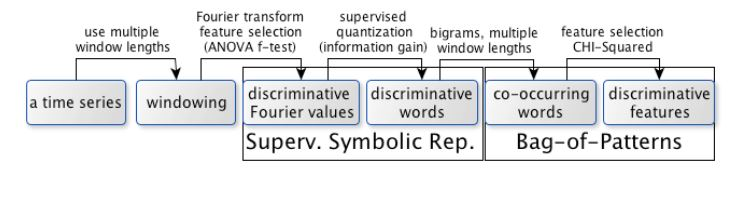
\includegraphics[scale = 0.5]{WEASELFlow.JPG}
    \centering
    \caption{WEASEL Pipeline: Feature extraction using a novel supervised symbolic representation, and a novel bag-of-patterns model \cite{schafer2017fast}}
    \label{Img:WEASELFlow}
\end{figure}

% Feature Extraction
WEASEL, like BOSS, transforms extracted windows from a time series into words using an alphabet of size $c$.
They identify two main drawbacks for SFA, and introduce a new supervised symbolic representation technique which is based on SFA but overcomes the drawbacks.
The first drawback of SFA is that it acts like a low pass filter and excludes the high frequency components from the Fourier transformation,
which might discard important features in some scenarios. The other drawback, is that SFA defines the boundaries of bins during quantization
independent of the class labels; which might cause SFA words of equal frequencies to appear unnecessarily in multiple classes.
In order to over come the drawbacks of SFA, WEASEL follows two steps;
discriminative approximation using ANOVA F-test and discriminative quantization using information gain.

% Feature Extraction - approximation
As mentioned earlier, approximation involves representing a time series of length $n$ with a shorter, yet informative, representation of length $l$ by applying a Fourier transformation.
WEASEL aims at keeping the best class separating $l$, real and imaginary, Fourier coefficients by applying a one-way ANOVA F-test.
The test verifies the hypothesis that the means of two or more distributions/groups differ from each other \cite{lowry2014concepts}.
This can be tested by comparing two variances; the variance between groups and the variance within the groups.
Using the notations in \cite{schafer2017fast}, \emph{mean square between} ($MS_{B}$) and \emph{mean square within} ($MS_{W}$) respectively.
The F-values is then calculated as :
\begin{equation}
    F= \frac{MS_{B}}{MS_{W}}
\end{equation}
Then $l$ coefficients with the highest F-values are kept; as these represent features which have big differences between the classes (high $MS_{B}$) and
small differences within the same class (low $MS_{W}$).

% Feature Extraction - quantization
After that, discretization is carried out to set the split thresholds for each of the extracted Fourier value.
Discretization involves a binning process, where each Fourier value is divided into a number of bins.
Each bin is represented by an upper and a lower boundary, and assigned a letter from an alphabet $c$.
Previous quantization techniques used equi-depth or equi-width binning, but these techniques are solely based on values and ignore the distribution of classes.
WEASEL applies a binning technique based on IG; assuring that for each partition the majority of the values would belong to the same class.
Figure \ref{Img:WEASEL_FEATURE} demonstrates the feature selection and quantization processes for WEASEL.

\begin{figure}[!htbp]
    \captionsetup{justification=raggedright}
    \centering
    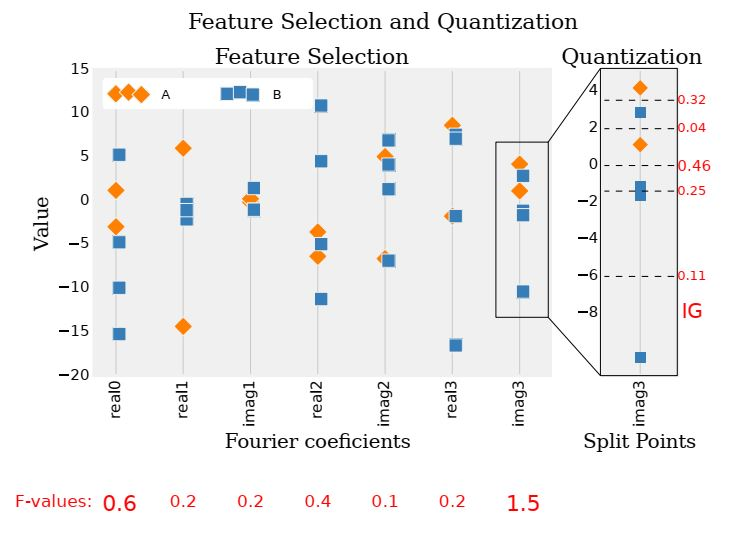
\includegraphics[scale = 0.5]{WEASEL_FEATURE.JPG}
    \centering
    \caption{On the left: Distribution of Fourier coefficients for a sample dataset. The high F-values on imag3 and real0 (red text at bottom) should be selected to best separate the samples from class labels ’A’ and ’B’. On the right: Zoom in on imag3. Information gain splitting is applied to find the best bins for the subsequent quantization. High information gain (IG) indicates pure (good) split points \cite{schafer2017fast}}
    \label{Img:WEASEL_FEATURE}
\end{figure}

% Feature Selection
The result of the feature extraction phase is a high dimensional feature vector with a dimensionality of $\mathcal{O}(min(Nn^{2},c^{l})$,
where $c$ is an alphabet, $l$ is the length of a word, $n$ is the total number of instances and $n$ is the length of the time series.
Since WEASEL uses bi-grams and $\mathcal{O}(n)$ window lengths, the dimensionality of the feature space increases to $\mathcal{O}(min(Nn^{2},c^{2l} \cdot n)$.
This enormous feature space is then reduced using a Chi-squared ($\chi^{2}$) test. Chi-squared tests is a statistical test used to determine if there is a significant difference
between the recognised frequencies and the expected frequencies of of a features within a group. This implies that features which have high ($\chi^{2}$) values are statistically
frequent in certain classes. By comparing the ($\chi^{2}$) values of features to a threshold, all features with scores lower than the threshold can be excluded from the faeture space.
This usually reduced the feature space by 30\% - 70\% and helped train the logistic regresion classifier in a timely manner.